% !TEX root = main.tex
\documentclass[letterpaper, 11pt]{extarticle}
% \usepackage{fontspec}

% ==================================================

% document parameters
% \usepackage[spanish, mexico, es-lcroman]{babel}
\usepackage[english]{babel}
\usepackage[margin = 1in]{geometry}

% ==================================================

% Packages for math
\usepackage{mathrsfs}
\usepackage{amsfonts}
\usepackage{amsmath}
\usepackage{amsthm}
\usepackage{amssymb}
\usepackage{physics}
\usepackage{dsfont}
\usepackage{esint}

% ==================================================

% Packages for writing
\usepackage{enumerate}
\usepackage[shortlabels]{enumitem}
\usepackage{framed}
\usepackage{csquotes}

% ==================================================

% Miscellaneous packages
\usepackage{float}
\usepackage{tabularx}
\usepackage{xcolor}
\usepackage{multicol}
\usepackage{subcaption}
\usepackage{caption}
\captionsetup{format = hang, margin = 10pt, font = small, labelfont = bf}

% Citation
\usepackage[round, authoryear]{natbib}

% Hyperlinks setup
\usepackage{hyperref}
\definecolor{links}{rgb}{0.36,0.54,0.66}
\hypersetup{
   colorlinks = true,
    linkcolor = black,
     urlcolor = blue,
    citecolor = blue,
    filecolor = blue,
    pdfauthor = {Author},
     pdftitle = {Title},
   pdfsubject = {subject},
  pdfkeywords = {one, two},
  pdfproducer = {LaTeX},
   pdfcreator = {pdfLaTeX},
   }

% \begin{document}
% Hello, world! This is a minimal document to test the preamble.
% \end{document}

\usepackage{listings} 
\usepackage{xcolor}

\definecolor{codegreen}{rgb}{0.12,0.6,0.33}
\definecolor{codegray}{rgb}{0.5,0.5,0.5}
\definecolor{codepurple}{rgb}{0.58,0,0.82}
\definecolor{codeblue}{rgb}{0,0.1,0.8}
\definecolor{backcolour}{rgb}{0.95,0.95,0.92}

\lstdefinestyle{pythonstyle}{
   backgroundcolor=\color{backcolour},
   commentstyle=\color{codegreen},
   keywordstyle=\color{codeblue}\bfseries,
   numberstyle=\tiny\color{codegray},
   stringstyle=\color{codepurple},
   basicstyle=\ttfamily\footnotesize,
   breakatwhitespace=false,
   breaklines=true,
   captionpos=b,
   keepspaces=true,
   numbers=left,
   numbersep=5pt,
   showspaces=false,
   showstringspaces=false,
   showtabs=false,
   tabsize=4,
   language=Python
}

% \usepackage{minted}

\usepackage{titlesec}
\usepackage[many]{tcolorbox}

% Adjust spacing after the chapter title
\titlespacing*{\chapter}{0cm}{-2.0cm}{0.50cm}
\titlespacing*{\section}{0cm}{0.50cm}{0.25cm}

% Indent 
\setlength{\parindent}{0pt}
\setlength{\parskip}{1ex}

% --- Theorems, lemma, corollary, postulate, definition ---
% \numberwithin{equation}{section}

\newtcbtheorem[]{problem}{Problem}%
    {enhanced,
    colback = black!5, %white,
    colbacktitle = black!5,
    coltitle = black,
    boxrule = 0pt,
    frame hidden,
    borderline west = {0.5mm}{0.0mm}{black},
    fonttitle = \bfseries\sffamily,
    breakable,
    before skip = 3ex,
    after skip = 3ex
}{problem}

\tcbuselibrary{skins, breakable}

% --- You can define your own color box. Just copy the previous \newtcbtheorm definition and use the colors of yout liking and the title you want to use.
% --- Basic commands ---
%   Euler's constant
\newcommand{\eu}{\mathrm{e}}

%   Imaginary unit
\newcommand{\im}{\mathrm{i}}

%   Sexagesimal degree symbol
\newcommand{\grado}{\,^{\circ}}

% --- Comandos para álgebra lineal ---
% Matrix transpose
\newcommand{\transpose}[1]{{#1}^{\mathsf{T}}}

%%% Comandos para cálculo
%   Definite integral from -\infty to +\infty
\newcommand{\Int}{\int\limits_{-\infty}^{\infty}}

%   Indefinite integral
\newcommand{\rint}[2]{\int{#1}\dd{#2}}

%  Definite integral
\newcommand{\Rint}[4]{\int\limits_{#1}^{#2}{#3}\dd{#4}}

%   Dot product symbol (use the command \bigcdot)
\makeatletter
\newcommand*\bigcdot{\mathpalette\bigcdot@{.5}}
\newcommand*\bigcdot@[2]{\mathbin{\vcenter{\hbox{\scalebox{#2}{$\m@th#1\bullet$}}}}}
\makeatother

%   Hamiltonian
\newcommand{\Ham}{\hat{\mathcal{H}}}

%   Trace
\renewcommand{\Tr}{\mathrm{Tr}}

% Christoffel symbol of the second kind
\newcommand{\christoffelsecond}[4]{\dfrac{1}{2}g^{#3 #4}(\partial_{#1} g_{#2 #4} + \partial_{#2} g_{#1 #4} - \partial_{#4} g_{#1 #2})}

% Riemann curvature tensor
\newcommand{\riemanncurvature}[5]{\partial_{#3} \Gamma_{#4 #2}^{#1} - \partial_{#4} \Gamma_{#3 #2}^{#1} + \Gamma_{#3 #5}^{#1} \Gamma_{#4 #2}^{#5} - \Gamma_{#4 #5}^{#1} \Gamma_{#3 #2}^{#5}}

% Covariant Riemann curvature tensor
\newcommand{\covariantriemanncurvature}[5]{g_{#1 #5} R^{#5}{}_{#2 #3 #4}}

% Ricci tensor
\newcommand{\riccitensor}[5]{g_{#1 #5} R^{#5}{}_{#2 #3 #4}}

\begin{document}

\textsf{\LARGE{\textbf{Take-home exam 2}}}

\normalsize{\textit{Dynamical Systems}}

\vspace{1ex}

\textsf{\textbf{Student:}} \text{Males-Araujo Yorlan}, 
\href{mailto:yorlan.males@yachaytech.edu.ec}{\texttt{yorlan.males@yachaytech.edu.ec}}\\
\textsf{\textbf{Lecturer:}} \text{Mario Cosenza}, 
\href{mcosenza@yachaytech.edu.ec}{\texttt{mcosenza@yachaytech.edu.ec}}

Yachay Tech, \today.

\vspace{2ex}



\begin{problem}{Superestable orbit}{problem-label-2}

Let $r_n^*$ be the parameter value of a quadratic map $f_r(x)$ for which there
exists a superstable orbit of period $2^n$.

\begin{enumerate}[(a)]
    \item Consider an arbitrary function $h(r_n)$ evaluated at $r_n^*$. Show that, 
    for $n \gg 1$, $h(r_n)$ satisfies the relation [1]:
    \[
        \frac{[h(r_n^*)-h(r_{\infty})]\delta^n}{h'(r_{\infty})} = \text{cte.}
    \]
    \item Show that for $ n \gg 1$, [1]
    \[
        (r_n^*-r_{\infty})\delta^n \propto \frac{\delta^2}{\delta -1}.
    \]
\end{enumerate}
\end{problem}

\begin{enumerate}[(a)]
    \item We start by expanding the function $h(r_n^*)$ around $r_{\infty}$:
    \[
        h(r_n^*) = h(r_{\infty}) + h'(r_{\infty})(r_n^*-r_{\infty}) + O((r_n^*-r_{\infty})^2).
    \]
    For large $n$, we can neglect higher-order terms:
    \[
        h(r_n^*) - h(r_{\infty}) \approx h'(r_{\infty})(r_n^*-r_{\infty}).
    \]
    Now, we can use the relation for the superstable orbit:
    \[
        r_n^* - r_{\infty} = C \delta^{-n},
    \]
    where $C$ is a constant. Substituting this into the previous equation gives us
    \[
        h(r_n^*) - h(r_{\infty}) \approx h'(r_{\infty})C\delta^{-n},
    \]
    and rearranging yields
    \[
    \boxed{
        \frac{[h(r_n^*)-h(r_{\infty})]\delta^n}{h'(r_{\infty})} = C
    }.
    \]
    \item We can express $r_n^* - r_{\infty}$ as a telescopic series,
    \[
        r_n^* - r_{\infty} = (r_{n}^* - r_{n+1}^*) + (r_{n+1}^* - r_{n +2}^*) + \ldots = \sum_{j=0}^{\infty} (r_{n+j}^* - r_{n+j+1}^*).
    \]
    Let $\Delta_n = r_{n+j}^* - r_{n+j+1}^*$, so that $\Delta_{n+1} = \Delta_n/\delta$. We can then write
    \[
        r_n^* - r_{\infty} = \Delta_n \sum_{j=0}^{\infty} \frac{1}{\delta^j} = \Delta_n \frac{\delta}{\delta - 1},
    \]
    using geometric series properties. The last step is given by $\Delta_n = \Delta_1/\delta^{n-1}$, where $\Delta_1$ is a constant. Thus,
    \[
        r_n^* - r_{\infty} = \frac{\Delta_1}{\delta^{n-1}} \frac{\delta}{\delta - 1} \implies \boxed{
            (r_n^*-r_{\infty})\delta^n \propto \frac{\delta^2}{\delta -1}
        }.
    \]

\end{enumerate}

\begin{problem}{Schwarz derivative}{problem-label-3}

Consider the logarithmic map $x_{n+1}=f(x_n)=b+\log|x_n|$.

\begin{enumerate}[(a)]
    \item Calculate the Schwarz derivative of this map. [1]
    \item Show that the Lyapunov exponent for this map can be expressed as [1]
    \[
        \lambda = b - \frac{1}{n}\sum_{j=1}^{n}x_j.
    \] 
\end{enumerate}
\end{problem}

\begin{enumerate}[(a)]
    \item The Schwarz derivative is given by
    \[
        Sf(x) = \frac{f'''}{f'} - \frac{3}{2}\left(\frac{f''}{f'}\right)^2.
    \]
    So we start by calculating all the derivatives,
    \begin{align*}
        f'(x) &= \frac{1}{x}, \\
        f''(x) &= -\frac{1}{x^2}, \\
        f'''(x) &= \frac{2}{x^3},
    \end{align*}
    substituting them in the relation, and simplifying we get
    \begin{align*}
            Sf(x) &= \frac{2}{x^3}\frac{x}{1} - \frac{3}{2}\left(-\frac{1}{x^2}\frac{x}{1}\right)^2 \\
                  &= \frac{2}{x^2} - \frac{3}{2}\left(-\frac{1}{x}\right)^2 \\
                  &= \frac{2}{x^2} - \frac{3}{2x^2} \\
                  &= \frac{1}{2x^2}.
    \end{align*}

    In conclusion, the Schwarz derivative is \textit{always positive}, and it is given by
    \[
        \boxed{
            Sf(x) = \frac{1}{2x^2}.
        }
    \]

    \item The Lyapunov exponent is given by
    \[
        \lambda = \lim_{n\to\infty}\frac{1}{n}\sum_{j=0}^{n-1}\log|f'(x_j)|.
    \]
    Since we already have the expression for $f'(x)$, we can just substitute it and simplify again:
    \begin{align*}
        \lambda &= \lim_{n\to\infty}\frac{1}{n}\sum_{j=0}^{n-1}\log\left|\frac{1}{x_j}\right| \\
                &= \lim_{n\to\infty}\frac{1}{n}\sum_{j=0}^{n-1}-\log|x_j|.
    \end{align*}
    Now, we can use the map to express $\log|x_j|$ in terms of $b$ and $x_{j-1}$:
    \begin{align*}
        \lambda &= \lim_{n\to\infty}\frac{1}{n}\sum_{j=0}^{n-1}-\log|x_j| \\
                &= \lim_{n\to\infty}\frac{1}{n}\sum_{j=0}^{n-1}(b - x_{j+1}) \\
                &= \lim_{n\to\infty}\frac{1}{n}\sum_{i=1}^{n}(b - x_{i}). \\
    \end{align*}
    Using properties of summation and limits, we can get $b$ out:
    \begin{align*}
        \lambda &= \lim_{n\to\infty}\frac{1}{n}\sum_{i=1}^{n}b - \lim_{n\to\infty}\frac{1}{n}\sum_{i=1}^{n}x_i \\
                &= \lim_{n\to\infty}\frac{nb}{n} - \lim_{n\to\infty}\frac{1}{n}\sum_{i=1}^{n}x_i \\
                &= b - \lim_{n\to\infty}\frac{1}{n}\sum_{i=1}^{n}x_i.
    \end{align*}

    Finally, for large $n$, we can write the expression as:
    \[
    \boxed{
        \lambda = b - \frac{1}{n}\sum_{j=1}^{n}x_i.
    }
    \]

\end{enumerate}

\begin{problem}{Bifurcation diagram}{problem-label-4}

Consider the following map for $x_n \in [0,1]$, depending on two real parameters $s$ and $c$,
\[
    x_{n+1} = f(x_n) = |\tanh[s(x_n-c)]|.
\]
Obtain the bifurcation diagram of $x_n$ as a function of $c \in [0,1]$ with fixed value $s=1.3$. [1]

\end{problem}

We reused the code from the previous take-home exam to get the bifurcation diagram. The only
thing we needed to change was the map function, which is now:

\begin{lstlisting}[style=pythonstyle]
# Map 
def tanh_map(x, c):
    return abs(np.tanh(1.3 * (x - c))
\end{lstlisting}

The result shows \textit{inverse period-doubling} for $c \in [0, 1]$, and it indicates
that the Schwarz derivative should be positive. 
The bifurcation diagram is shown in Figure \ref{fig:1a}.
\begin{figure}[!ht]
    \centering
    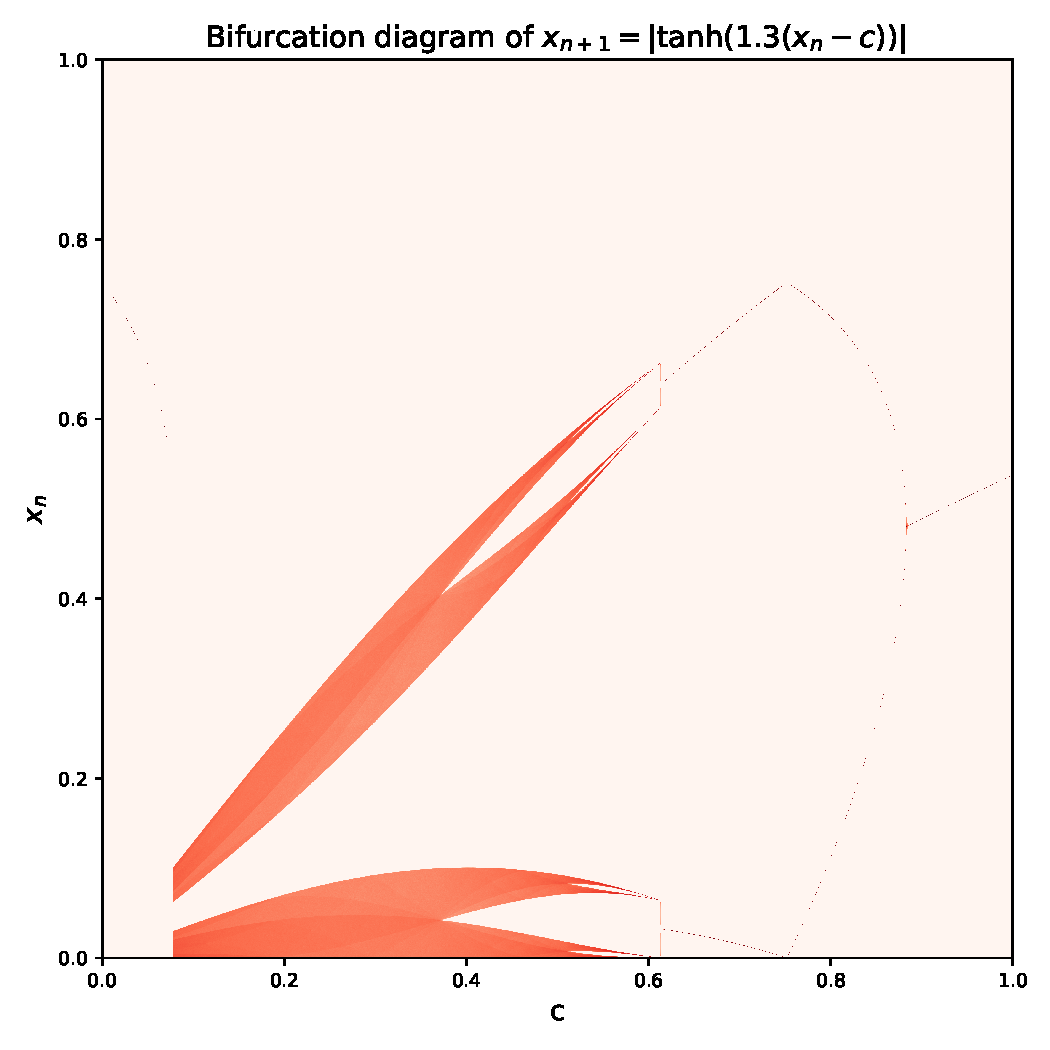
\includegraphics[scale=0.65]{images/tanh.pdf}
    \captionof{figure}{Inverse period-doubling for $s=1.3$.}
    \label{fig:1a}
\end{figure}

\begin{problem}{Lyapunov exponent}{problem-label-5}

Consider the following map for $x_n \in [0,1]$:
\[
    x_{n+1} = f(x_n) = \begin{cases}
        (1+\epsilon)x_n + x_n^2, & \text{if } x_n < x^*, \\
        1-x_n, & \text{if } x_n \geq x^*,
    \end{cases}
\]
where $x^*$ is the solution of $(1+\epsilon)x_n + x_n^2 = 1$.

\begin{enumerate}[(a)]
    \item Calculate the Lyapunov exponent versus $\epsilon \in [-0.4, 0.4]$. [1]
    \item Describe the route to chaos exhibited by this map on such interval. [1]

\end{enumerate}
\end{problem}

\begin{enumerate}[(a)]
    \item Again, we can use the same code as before but with some modifications.
    The map function and its derivative are given by:

    \newpage

    \begin{lstlisting}[style=pythonstyle]
    # Map
    def piecewise_map(x, eps, x_star):
        if x < x_star:
            return (1 + eps) * x + x**2
        else:
            return 1 - x
        
    # Derivative
    def derivative(x, eps, x_star):
        if x < x_star:
            return 1 + eps + 2 * x
        else:
            return -1
    \end{lstlisting}

    where \texttt{x\_star} has been previously calculated for each $\epsilon$.
    The result is shown in Figure \ref{fig:2a}.
    \begin{figure}[!ht]
        \centering
        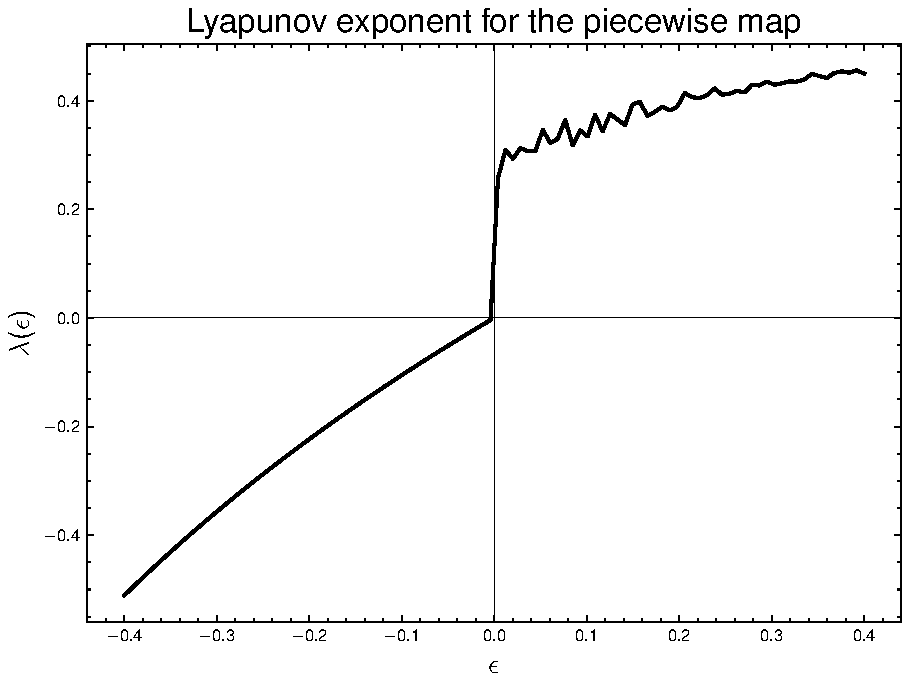
\includegraphics[scale=0.65]{images/piecewise_lya.pdf}
        \captionof{figure}{Evolution of the piecewise map for $\epsilon \in [-0.4, 0.4]$.}
        \label{fig:2a}
    \end{figure}

    The Lyapunov exponent is mostly negative for $\epsilon < 0$ and positive for $\epsilon > 0$, which
    suggests the map is chaotic for $\epsilon > 0$. The transition to chaos is not smooth at all: there's a 
    sudden and rapid change at $\epsilon \approx 0$.
    \item Of all the routes to chaos we have studied, the one that adjusts better to the behavior of this map is
    \textit{intermittency} because of the very rapid transition from periodic orbits to chaos. The Lyapunov exponent goes from negative
    to positive extremely quickly.
\end{enumerate}

\begin{problem}{Not period-doubling}{problem-label-6}
Consider the following map for $x_n \in [0,1],$
\[
    x_{n+1} = f(x_n) = \frac{1-b^{x_n(1-x_n)}}{1-b^{1/4}}
\]
\begin{enumerate}[(a)]
    \item Is this map unimodal for $b \in (0,1)$? [1]
    \item Plot the bifurcation diagram of $x_n$ on the interval $b \in (0,1)$ and $x_n \in [0,1]$.
    Why does this map not show period doubling? [1]
    \item Find the Lyapunov exponent for $b \in (0,1)$. [1]
\end{enumerate}
\end{problem}

\begin{enumerate}[(a)]
    \item One way to see if the map is unimodal is to plot $f(x_n)$ versus $x_n$ for different values
    of $b$, and then \textit{visually} check if the function has one maximum or minimum. We did it
    for many $b$'s and the results are shown in Figure \ref{fig:3a}.
    \begin{figure}[!ht]
        \centering
        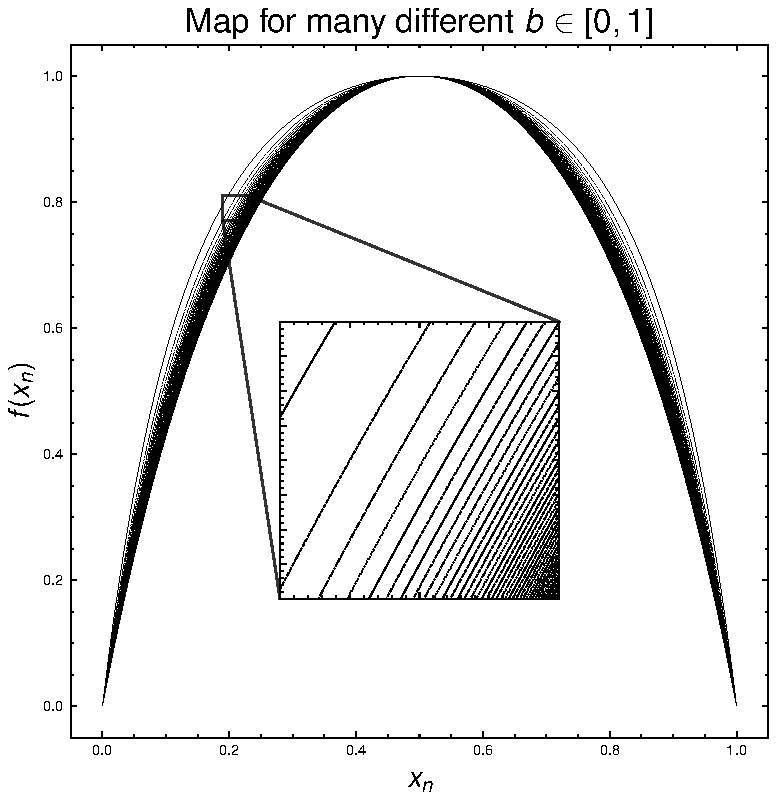
\includegraphics[scale=0.65]{images/unimodal.pdf}
        \captionof{figure}{Plots of $f(x_n)=\frac{1-b^{x_n(1-x_n)}}{1-b^{1/4}}$ for $b \in (0,1)$.}
        \label{fig:3a}
    \end{figure}

    There is only one maximum, which suggests the map in unimodal. However, a more rigorous way to
    check it is to calculate the derivative of the map and see if it has only \textit{one root}. So, the
    derivative is given by
    \[
    f'(x) = \frac{(1-2x)b^{x(1-x)}\log(b)}{(1-b^{1/4})}
    \]
    and it effectively has one root only: $x = 1/2$. Thus, \boxed{\text{the map is indeed unimodal.}}

    \item As always, reusing code but changing the map:
    \begin{lstlisting}[style=pythonstyle]
    # Map
    def frac_map(x, b):
        num = 1 - b**(x * (1 - x))
        den = 1 - b**(1/4) + 1e-10 # Avoid division by zero
        return num/den
    \end{lstlisting}
    We obtained the results shown in Figure \ref{fig:3b}.
    \newpage
    \begin{figure}[!ht]
        \centering
        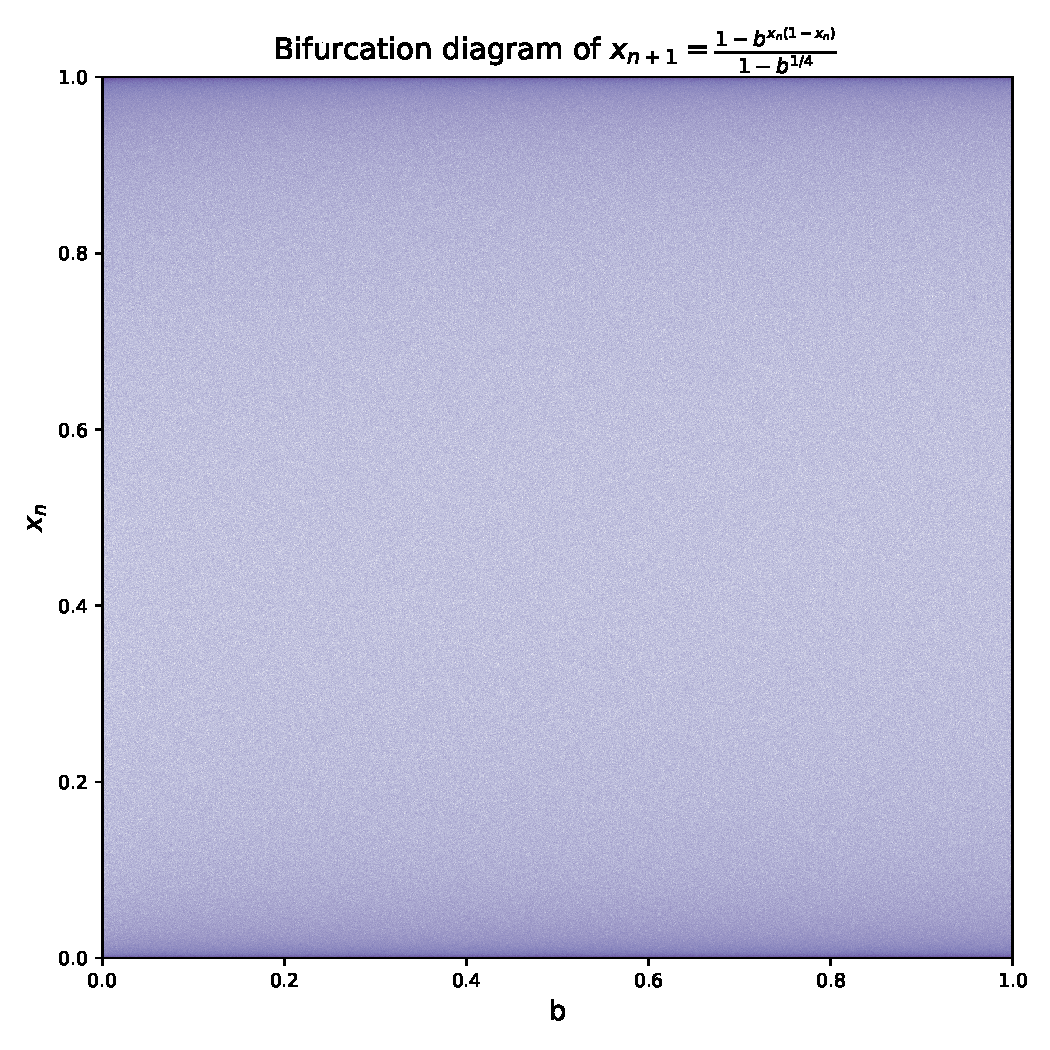
\includegraphics[scale=0.65]{images/b_power.pdf}
        \captionof{figure}{Pure chaos for $b \in (0,1)$.}
        \label{fig:3b}
    \end{figure}

    The map is chaotic from start to finish for $b \in (0,1)$. It covers 
    the full range of $x_n \in [0,1]$, but the diagram seems to be uniform, that is, 
    it doesn't change at any point. It's quite interesting to see this kind of behavior.

    \item We were expecting a positive and constant Lyapunov exponent because of the previous part,
    and that's exactly what we got. In order to do it, we had first to compute and code
    the derivative of the map:
    \begin{lstlisting}[style=pythonstyle]
    # Derivative
    def frac_derivative(x, b):
        num = (1 - 2 * x) * b**(x * (1 - x)) * np.log(b)
        den = - (1 - b**(1/4)) + 1e-10 # Again, avoid division by zero
        return num/den
    \end{lstlisting}
    Then, we ran the code and obtained the results shown in Figure \ref{fig:3c}.
    \newpage
    \begin{figure}[!h]
        \centering
        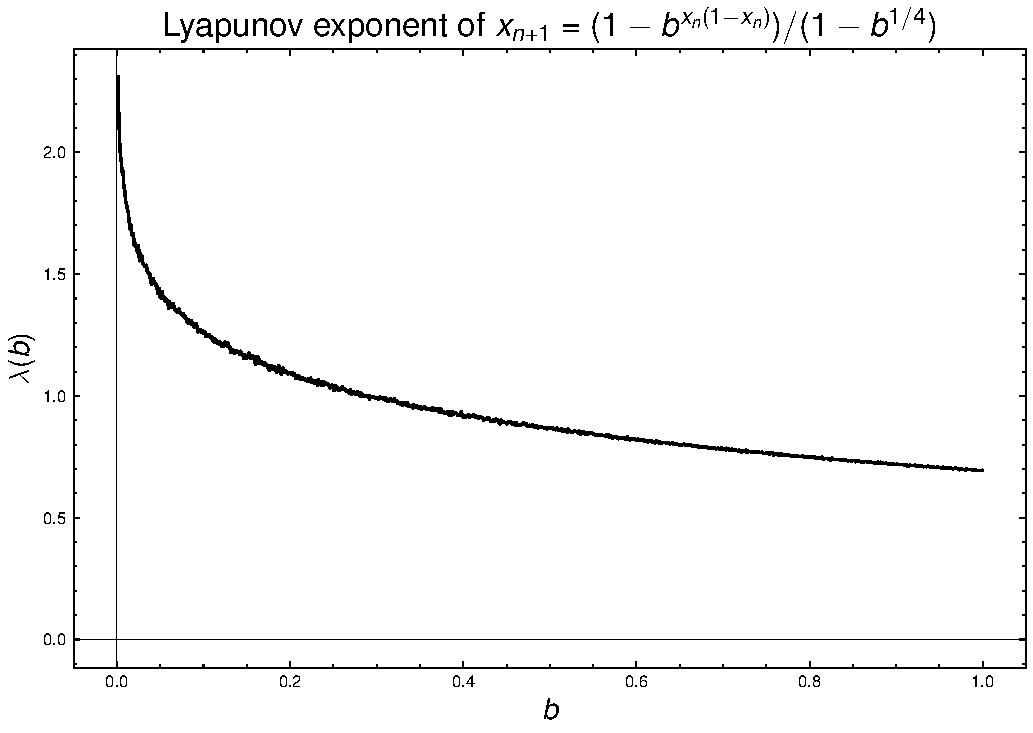
\includegraphics[scale=0.65]{images/frac_lya.pdf}
        \captionof{figure}{Lyapunov exponent for $b \in (0,1)$.}
        \label{fig:3c}
    \end{figure}

    It is indeed positive for all $b \in (0,1)$, which goes hand in hand with its
    bifurcation diagram.
\end{enumerate}


% \newpage
% \vspace{0.1ex}

% \bibliographystyle{apalike}
% \bibliography{references}

\end{document}